%**************************************************************************************
% License:
% CC BY-NC-SA 4.0 (http://creativecommons.org/licenses/by-nc-sa/4.0/)
%**************************************************************************************
% Figures and every number on these slides come from figs/src/generate_ad_figures.py
% (report in figs/src/generate_ad_figures-report.txt) and figs/src/page_numbers.js.

\documentclass{beamer}
\setbeameroption{hide notes}

\mode<presentation> {

\usetheme{Madrid}

% Burnt orange
\definecolor{burntorange}{rgb}{0.8, 0.33, 0.0}
\colorlet{beamer@blendedblue}{burntorange}
% Pale yellow
\definecolor{paleyellow}{rgb}{1.0, 1.0, 0.953}
\setbeamercolor{background canvas}{bg=paleyellow}
% Secondary and tertiary palette
\setbeamercolor*{palette secondary}{use=structure,fg=white,bg=burntorange!80!black}
\setbeamercolor*{palette tertiary}{use=structure,fg=white,bg=burntorange!60!black}

% Keep navigation symbols out of the content area.
\setbeamertemplate{navigation symbols}{}
}

\usepackage{amsmath}
\DeclareMathOperator*{\argmin}{arg\,min}
\DeclareMathOperator{\diag}{diag}
\DeclareMathOperator{\sign}{sign}
\DeclareMathOperator{\relu}{relu}
\usepackage{bm}
\usepackage{booktabs} % Allows the use of \toprule, \midrule and \bottomrule in tables
\usepackage{array}
\newcolumntype{L}[1]{>{\raggedright\arraybackslash}p{#1}}
\usepackage{graphicx} % for figures
\usepackage{xcolor}
\usepackage{hyperref}

\AtBeginSection[]{
	\begin{frame}[shrink=5]{Outline}
		\tableofcontents[
		currentsection,      % highlight the current section
		hideallsubsections   % show only section titles
		]
	\end{frame}
}

%----------------------------------------------------------------------------------------
%	TITLE PAGE
%----------------------------------------------------------------------------------------
\title[Automatic Differentiation]{Automatic Differentiation and Optimization}
\author{Krishna Kumar} % name
\institute[UT Austin] % institution
{
University of Texas at Austin \\
\medskip
\textit{
  \url{krishnak@utexas.edu}} % Your email address
}
\date{} % Date, can be changed to a custom date

\begin{document}

\begin{frame}[shrink=5]
\titlepage % title page as the first slide
\end{frame}


%----------------------------------------------------------------------------------------
% slides
%----------------------------------------------------------------------------------------

\section{Derivatives of a Program}

%------------------------------------------------
\begin{frame}
\frametitle{Learning Objectives}
\begin{itemize}
\item Differentiate a program with forward mode and with reverse mode
\item Count the sweeps and the memory that each mode needs
\item Differentiate a time-stepping simulator, and relate reverse mode to the adjoint method
\item Compare the steps of gradient descent, Adam, Newton, and L-BFGS
\item Explain why the gradient depends on the scaling of the parameters
\item Use subgradients for losses with kinks
\end{itemize}
\vspace{0.3cm}
\centering
\href{https://colab.research.google.com/github/kks32-courses/sciml/blob/main/docs/06-ad/06-ad.ipynb}{\beamergotobutton{AD notebook}}
\href{https://kks32-courses.github.io/sciml/06-ad/gradients-and-optimizers.html}{\beamergotobutton{Gradients and optimizers}}
\href{https://colab.research.google.com/github/kks32-courses/sciml/blob/main/docs/06-ad/inverse-updates.ipynb}{\beamergotobutton{Inverse updates}}
\href{https://colab.research.google.com/github/kks32-courses/sciml/blob/main/docs/06-ad/subgradients.ipynb}{\beamergotobutton{Subgradients}}
\end{frame}

%------------------------------------------------
\begin{frame}
\frametitle{Forward and inverse problems}
Here is a simulator.
It takes parameters, such as a friction angle $\phi$, a stiffness $E$, or a permeability $k$, and returns results.
\begin{center}
\includegraphics[width=0.72\textwidth,height=0.3\textheight,keepaspectratio]{forward-inverse.png}
\end{center}
The forward problem runs the simulator.
The inverse problem starts from measured results and asks for the parameters that produced them.
\bigskip

We answer it by minimizing the mismatch between the simulator and the measurements.
How do we get the derivative of that mismatch with respect to the parameters?
\end{frame}

%------------------------------------------------
\begin{frame}
\frametitle{The projectile}
Here is a ball launched with speed $v$ at an angle $a$.
We observe the top of its arc, $\mathbf y^*$, and we want the $v$ and $a$ that produced it.
\[
\mathbf y(v,a)=\left(\frac{v^2\sin 2a}{2g},\ \frac{v^2\sin^2 a}{2g}\right),
\qquad
L(v,a)=\tfrac12\,\lVert \mathbf y(v,a)-\mathbf y^*\rVert^2 .
\]
\begin{center}
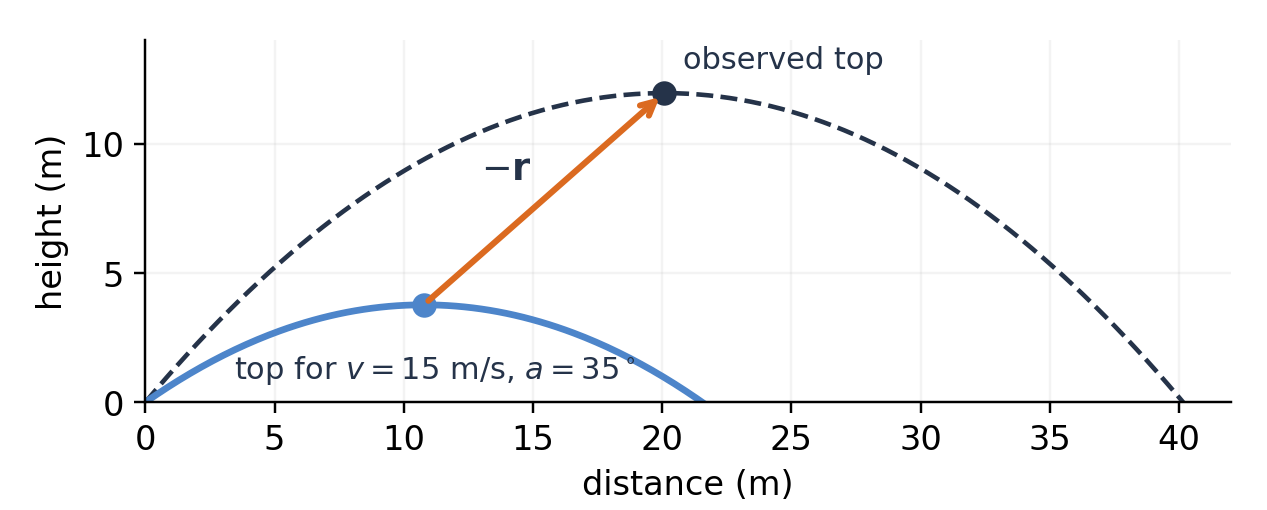
\includegraphics[width=0.85\textwidth,height=0.36\textheight,keepaspectratio]{figs/projectile-arcs.png}
\end{center}
The observed top is at $(20.08,\,11.96)$ m.
A first guess, $v=15$ m/s and $a=35^\circ$, puts the top at $(10.78,\,3.77)$ m, and the loss is $76.8$.
Which way should we change $v$ and $a$?
\end{frame}

%------------------------------------------------
\begin{frame}
\frametitle{Differentiating a program}
We need $\partial L/\partial v$ and $\partial L/\partial a$, and the loss is a program.
There are three ways to differentiate it.
\bigskip

\begin{center}
\footnotesize
\begin{tabular}{llll}
\toprule
Method & Works on & Error & Cost, $n$ parameters\\
\midrule
Finite differences & program runs & truncation, rounding & $n+1$ runs\\
Symbolic & a formula & none & a long formula\\
Automatic & each operation & rounding & 1 or $n$ sweeps\\
\bottomrule
\end{tabular}
\end{center}
\bigskip

Automatic differentiation applies the chain rule to each operation as the program runs.
It returns a number, the derivative at the current parameters, and it never builds a formula.
\end{frame}

%------------------------------------------------
\begin{frame}
\frametitle{Finite differences}
The obvious move changes one parameter by $h$ and runs the program again,
\[
\frac{\partial L}{\partial v}\approx\frac{L(v+h,a)-L(v,a)}{h}.
\]
\begin{columns}[T]
\begin{column}{0.56\textwidth}
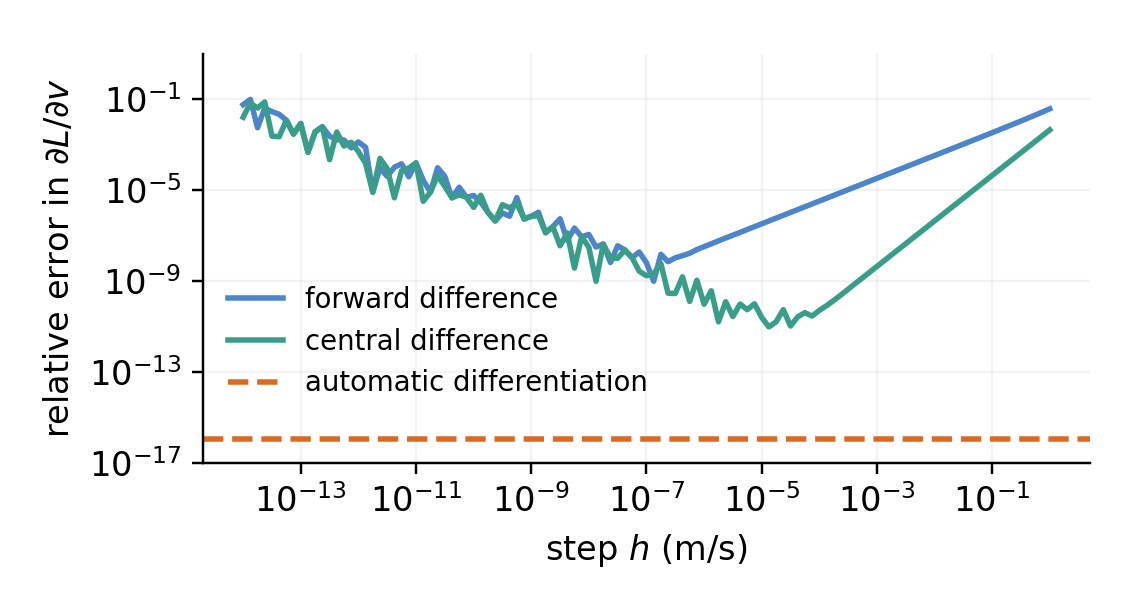
\includegraphics[width=\linewidth]{figs/fd-error.png}
\end{column}
\begin{column}{0.42\textwidth}
\small
A large $h$ leaves a truncation error that grows with $h$.
A small $h$ subtracts two nearly equal numbers, and the rounding error grows like $1/h$.
\medskip

The best forward difference has a relative error of $10^{-9}$.
The best central difference reaches $10^{-11}$.
\medskip

Each parameter costs one more run.
\end{column}
\end{columns}
\end{frame}

%------------------------------------------------
\begin{frame}
\frametitle{Symbolic differentiation}
A computer algebra system differentiates a formula.
Try it on the loop $l_{n+1}=4\,l_n(1-l_n)$ with $l_1=x$.
\begin{center}
\small
\begin{tabular}{lcccccc}
\toprule
$n$ & 2 & 3 & 4 & 5 & 6 & 7\\
\midrule
Operations in the formula for $l_n$ & 3 & 8 & 18 & 38 & 78 & 158\\
Operations in the formula for $dl_n/dx$ & 2 & 21 & 82 & 264 & 768 & 2096\\
Operations in the loop that computes $l_n$ & 3 & 6 & 9 & 12 & 15 & 18\\
\bottomrule
\end{tabular}
\end{center}
\medskip
The loop for $l_7$ runs 18 operations.
Its derivative, written as one formula, has 2096.
\bigskip

Automatic differentiation keeps the loop.
It adds a few operations to each pass, so its cost grows with the length of the program.
\note{Operation counts are SymPy's count\_ops on the expressions without simplification. Baydin et al. (2018) use the same iteration to show expression swell.}
\end{frame}

%------------------------------------------------
\section{Forward Mode}

%------------------------------------------------
\begin{frame}
\frametitle{A program as a list of operations}
Take a smaller function, $y=x_1^2+x_2$.
A program computes it one elementary operation at a time.
\begin{columns}[T]
\begin{column}{0.56\textwidth}
\includegraphics[width=\linewidth]{ad2.png}
\end{column}
\begin{column}{0.42\textwidth}
\[
\begin{aligned}
w_1&=x_1\\
w_2&=x_2\\
w_3&=w_1^2\\
w_4&=w_3+w_2\\
y&=w_4
\end{aligned}
\]
At $x_1=2$ and $x_2=3$ the list gives $w_3=4$ and $y=7$.
\end{column}
\end{columns}
\medskip
This list is the \textbf{tape}.
Every row is an operation whose derivative we know.
\end{frame}

%------------------------------------------------
\begin{frame}
\frametitle{Forward mode}
Carry a second number beside every value, the \textbf{tangent} $\dot w=\partial w/\partial x_1$.
Each row updates its tangent with the derivative of its own operation.
\begin{center}
\begin{tabular}{llcc}
\toprule
Row & Tangent rule & Value & Tangent\\
\midrule
$w_1=x_1$ & seed & 2 & 1\\
$w_2=x_2$ & seed & 3 & 0\\
$w_3=w_1^2$ & $\dot w_3=2w_1\,\dot w_1$ & 4 & 4\\
$w_4=w_3+w_2$ & $\dot w_4=\dot w_3+\dot w_2$ & 7 & 4\\
\bottomrule
\end{tabular}
\end{center}
One sweep down the tape gives $\partial y/\partial x_1=4$.
\bigskip

For $\partial y/\partial x_2$ we change the seed to $(\dot w_1,\dot w_2)=(0,1)$ and sweep again.
That sweep ends with $\dot w_4=1$.
\end{frame}

%------------------------------------------------
\begin{frame}
\frametitle{Dual numbers}
Forward mode needs no stored tape.
Replace every number by a pair $a+b\,\epsilon$, with the rule $\epsilon^2=0$.
\[
(a+b\epsilon)+(c+d\epsilon)=(a+c)+(b+d)\,\epsilon,
\qquad
(a+b\epsilon)(c+d\epsilon)=ac+(ad+bc)\,\epsilon .
\]
The product rule is built into the multiplication, and for any smooth $f$,
\[
f(x+\epsilon)=f(x)+f'(x)\,\epsilon .
\]
Try our function at $x_1=2+\epsilon$ and $x_2=3$,
\[
(2+\epsilon)^2+3=4+4\epsilon+\epsilon^2+3=7+4\,\epsilon .
\]
The first number is the value and the coefficient of $\epsilon$ is $\partial y/\partial x_1$.
The sweep costs a small multiple of the program itself.
\end{frame}

%------------------------------------------------
\begin{frame}
\frametitle{The cost of forward mode}
A forward sweep follows one direction in the inputs.
With the seed $\mathbf e_i$ it returns $J\,\mathbf e_i$, the column $i$ of the Jacobian $J=\partial\mathbf y/\partial\mathbf x$.
\bigskip

\begin{itemize}
\item A function of one input and many outputs needs one sweep.
\item Our projectile loss has two parameters and needs two sweeps.
\item The wave model later in the deck has 1000 unknown speeds and needs 1000 sweeps.
\end{itemize}
\bigskip

A loss has many inputs and one output.
Can one sweep return all of its partial derivatives?
\end{frame}

%------------------------------------------------
\section{Reverse Mode}

%------------------------------------------------
\begin{frame}
\frametitle{Reverse mode}
Run the program once and keep every value.
Then walk the tape backward with the \textbf{adjoint} $\bar w=\partial y/\partial w$.
\begin{columns}[T]
\begin{column}{0.47\textwidth}
\includegraphics[width=\linewidth]{ad6.png}
\end{column}
\begin{column}{0.51\textwidth}
\footnotesize
\begin{tabular}{@{}llc@{}}
\toprule
Row & Adjoint rule & Adjoint\\
\midrule
$w_4=w_3+w_2$ & seed & 1\\
$w_3=w_1^2$ & $\bar w_3=\bar w_4$ & 1\\
$w_2=x_2$ & $\bar w_2=\bar w_4$ & 1\\
$w_1=x_1$ & $\bar w_1=2w_1\,\bar w_3$ & 4\\
\bottomrule
\end{tabular}
\medskip

\small
The adjoint rule of a row needs the value stored in that row, here $w_1=2$.
\end{column}
\end{columns}
\medskip
One backward sweep gives the whole gradient, $(\partial y/\partial x_1,\ \partial y/\partial x_2)=(4,1)$.
\end{frame}

%------------------------------------------------
\begin{frame}
\frametitle{Jacobian products}
A program maps $n$ inputs to $m$ outputs, and its Jacobian $J$ has $m$ rows and $n$ columns.
Neither mode builds $J$.
Each one multiplies $J$ by a vector.
\begin{center}
\footnotesize
\begin{tabular}{lll}
\toprule
 & Forward mode & Reverse mode\\
\midrule
One sweep computes & $J\,\mathbf v$ & $J^T\mathbf u$\\
The vector is & a direction $\mathbf v$ in the inputs & weights $\mathbf u$ on the outputs\\
Sweeps for all of $J$ & $n$ & $m$\\
Memory & the tangents of the current row & every value on the tape\\
Suits & few inputs & few outputs\\
\bottomrule
\end{tabular}
\end{center}
\medskip
A loss has $m=1$.
One reverse sweep with $\mathbf u=1$ returns $J^T$, which is the gradient, for any number of parameters.
The price is the memory of the tape.
\end{frame}

%------------------------------------------------
\begin{frame}[fragile]
\frametitle{Reverse mode in PyTorch}
PyTorch records the tape while the program runs.
\begin{verbatim}
import torch

x1 = torch.tensor(2.0, requires_grad=True)
x2 = torch.tensor(3.0, requires_grad=True)

y = x1**2 + x2        # forward sweep, recorded
y.backward()          # backward sweep, seed 1

print(x1.grad, x2.grad)   # tensor(4.) tensor(1.)
\end{verbatim}
The flag \texttt{requires\_grad=True} marks the inputs.
The call \texttt{backward()} sets $\bar y=1$ and sweeps the tape from the last row to the first.
\medskip

In JAX, \texttt{jax.grad(f)} returns a function that runs the reverse sweep, and \texttt{jax.jvp} runs a forward sweep.
\end{frame}

%------------------------------------------------
\begin{frame}
\frametitle{The tape of the projectile loss}
Here is the loss of the projectile at $v=15$ m/s and $a=35^\circ$, one operation per row.
\begin{center}
\footnotesize
\renewcommand{\arraystretch}{0.9}
\begin{tabular}{rllrrr}
\toprule
Row & Variable & Operation & Value & Tangent, seed $v$ & Adjoint\\
\midrule
1 & $v$ & input & 15 & 1 & $-17.48$\\
2 & $a$ & input & 35 & 0 & $-2.814$\\
3 & $\theta$ & $a\,\pi/180$ & 0.6109 & 0 & $-161.2$\\
4 & $s$ & $\sin\theta$ & 0.5736 & 0 & $-282.5$\\
5 & $c$ & $\cos\theta$ & 0.8192 & 0 & $-122.4$\\
6 & $q$ & $v^2$ & 225 & 30 & $-0.5828$\\
7 & $p$ & $q\,s$ & 129.05 & 17.21 & $-1.016$\\
8 & $x$ & $p\,c/g$ & 10.776 & 1.437 & $-9.301$\\
9 & $z$ & $p\,s/(2g)$ & 3.773 & 0.503 & $-8.191$\\
10 & $r_1$ & $x-x^*$ & $-9.301$ & 1.437 & $-9.301$\\
11 & $r_2$ & $z-z^*$ & $-8.191$ & 0.503 & $-8.191$\\
12 & $L$ & $(r_1^2+r_2^2)/2$ & 76.80 & $-17.48$ & 1\\
\bottomrule
\end{tabular}
\end{center}
\small
The forward sweep ends in row 12 with $\partial L/\partial v$.
The backward sweep starts there and ends in rows 1 and 2 with both partial derivatives.
\end{frame}

%------------------------------------------------
\begin{frame}
\frametitle{The Jacobian and the residual}
The chain rule splits the gradient into a physics part and a mismatch part,
\[
\nabla L=J^T\mathbf r,\qquad J=\frac{\partial\mathbf y}{\partial(v,a)},\qquad \mathbf r=\mathbf y-\mathbf y^* .
\]
\begin{center}
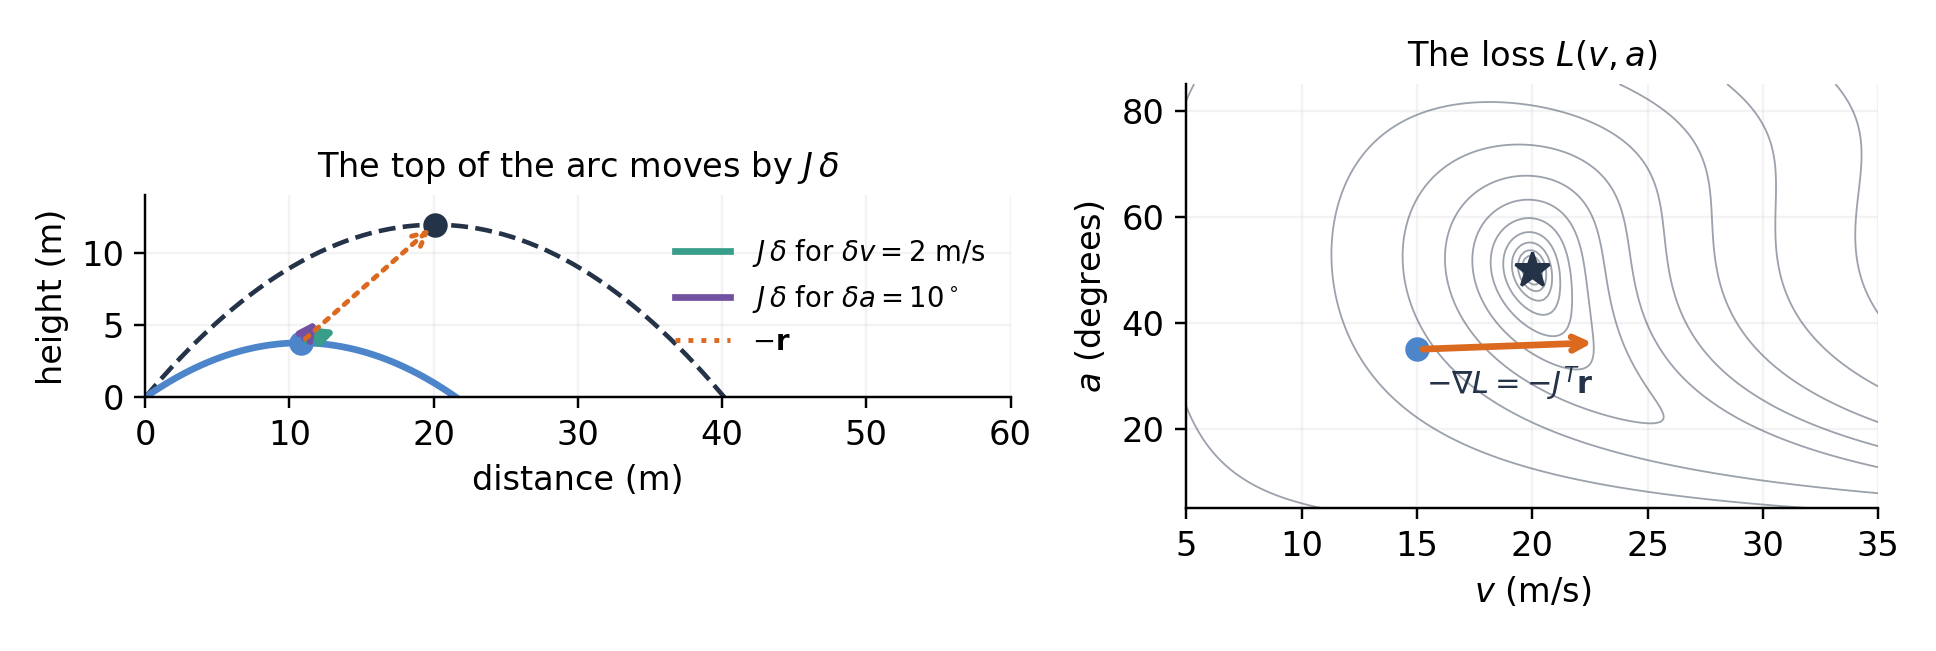
\includegraphics[width=\textwidth,height=0.42\textheight,keepaspectratio]{figs/projectile-gradient.png}
\end{center}
Rows 8 and 9 of the tape hold the top of the arc.
In a forward sweep they receive a column of $J$, the motion of the top when one parameter changes.
In the backward sweep they receive $\mathbf r$, and rows 1 and 2 return $J^T\mathbf r=(-17.48,\,-2.81)$.
\end{frame}

%------------------------------------------------
\begin{frame}
\frametitle{Units and the gradient}
Row 3 converts degrees to radians, and its adjoint multiplies by $\pi/180$.
\begin{columns}[T]
\begin{column}{0.5\textwidth}
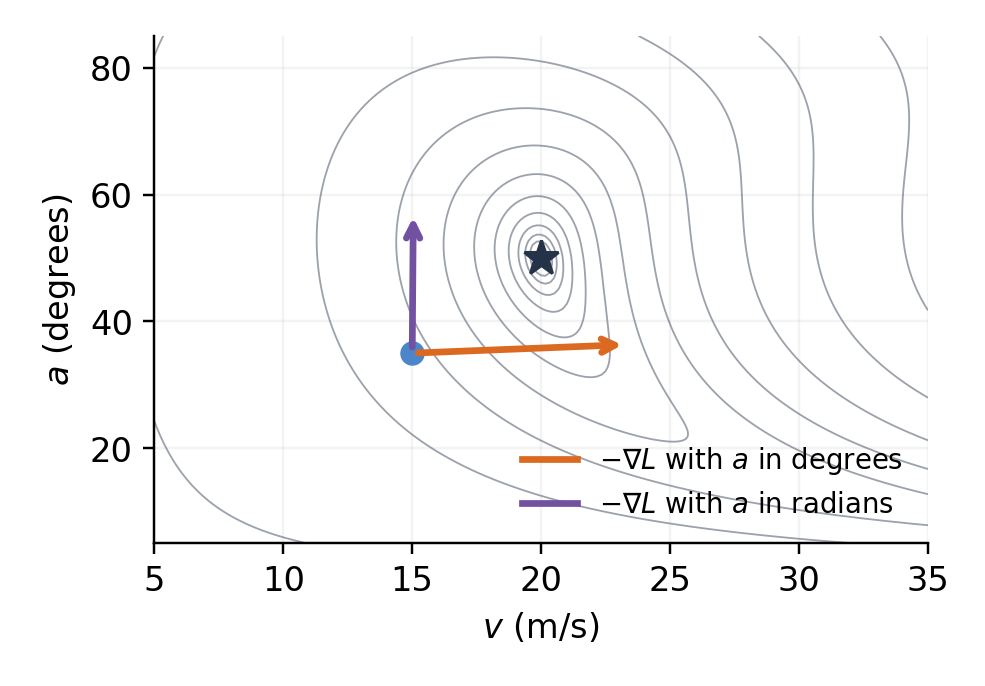
\includegraphics[width=\linewidth]{figs/units-gradient.png}
\end{column}
\begin{column}{0.48\textwidth}
\small
\begin{tabular}{lcc}
\toprule
Unit of $a$ & $\partial L/\partial v$ & $\partial L/\partial a$\\
\midrule
degrees & $-17.48$ & $-2.814$\\
radians & $-17.48$ & $-161.2$\\
\bottomrule
\end{tabular}
\medskip

The loss and the point are the same, and the direction $-\nabla L$ is different.
\medskip

The gradient has the units of $L$ divided by the units of each parameter.
A step $-\eta\,\nabla L$ inherits that scaling.
\medskip

Which scaling should the step use?
\end{column}
\end{columns}
\end{frame}

%------------------------------------------------
\section{Differentiating a Simulation}

%------------------------------------------------
\begin{frame}
\frametitle{Full-waveform inversion}
\begin{columns}[T]
\begin{column}{0.5\textwidth}
\includegraphics[width=\linewidth]{1dfwi.png}
\end{column}
\begin{column}{0.48\textwidth}
\small
A pulse travels down a soil column, and a sensor records the wave.
The wave speed $c(x)$ changes with depth,
\[
\frac{\partial^2u}{\partial t^2}=c^2\,\frac{\partial^2u}{\partial x^2}.
\]
We want the $c(x)$ whose simulated wave matches the recorded one.
\end{column}
\end{columns}
\medskip
Central differences advance the wave one step, with $C_i=c_i\,\Delta t/\Delta x$,
\[
u_i^{n+1}=2u_i^n-u_i^{n-1}+C_i^2\,(u_{i+1}^n-2u_i^n+u_{i-1}^n).
\]
The notebook uses 1000 grid points and 5000 time steps.
\end{frame}

%------------------------------------------------
\begin{frame}
\frametitle{The time loop on the tape}
The notebook compares the wave at the final time with the target, $L(\mathbf c)=\lVert\mathbf u^{N}(\mathbf c)-\mathbf u_{\text{target}}\rVert$.
The program is a loop, and its tape is the loop written out, one block of rows per time step.
\bigskip

\begin{center}
\begin{tabular}{ll}
\toprule
Method & Cost of $\partial L/\partial\mathbf c$ for 1000 speeds\\
\midrule
Finite differences & 1001 simulations\\
Forward mode & 1000 sweeps\\
Reverse mode & one sweep forward and one sweep backward\\
\bottomrule
\end{tabular}
\end{center}
\bigskip

The backward sweep needs the wave at every step.
That is $5000\times1000$, or 5 million stored values for each field.
\bigskip

Can we get the gradient from one backward solve without the tape?
\end{frame}

%------------------------------------------------
\begin{frame}
\frametitle{The adjoint equation}
Take the smallest example, $\dot y=-k\,y$ with $y(0)=y_0$, and the cost $J=\int_0^T (y-d)^2\,dt$.
Let $p(t)$ be the change in $J$ caused by a unit push on the state at time $t$.
It satisfies
\[
-\dot p=-k\,p+2\,(y-d),\qquad p(T)=0,
\]
and the gradients are $\ \dfrac{dJ}{dk}=-\displaystyle\int_0^T p\,y\,dt\ $ and $\ \dfrac{dJ}{dy_0}=p(0)$.
\begin{center}
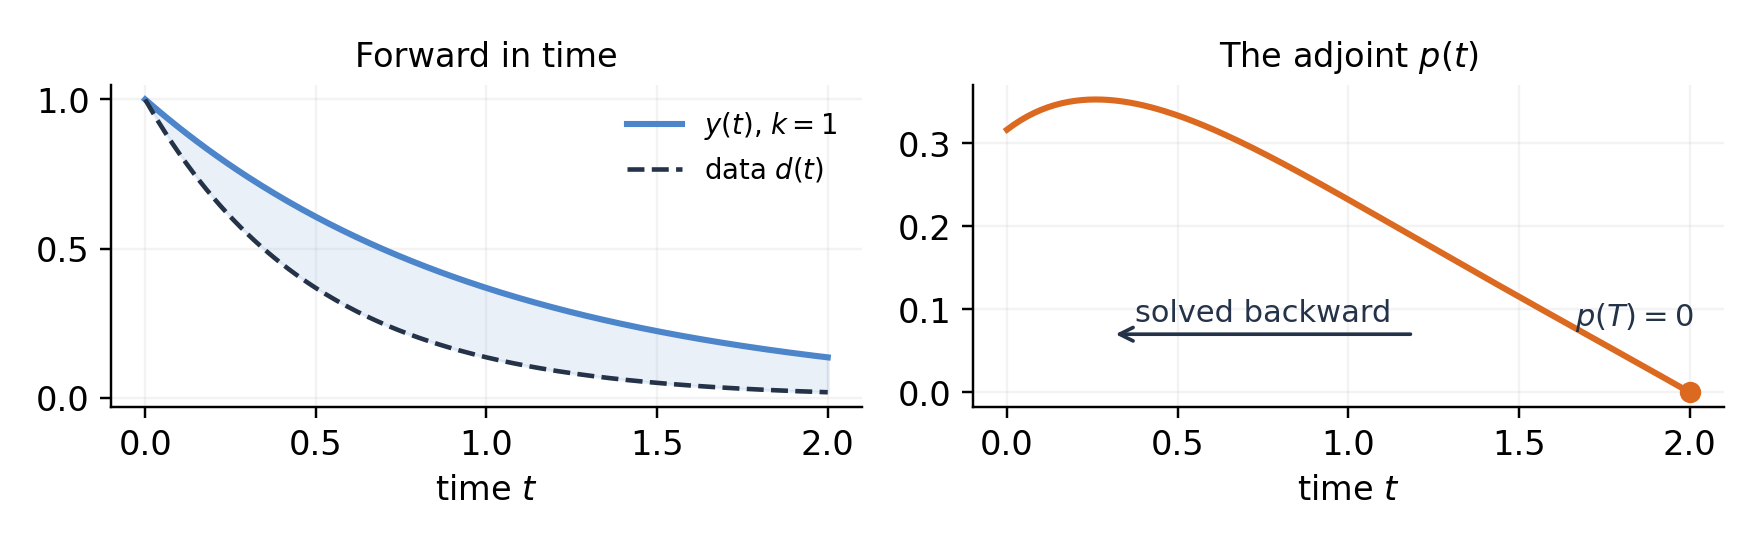
\includegraphics[width=0.92\textwidth,height=0.36\textheight,keepaspectratio]{figs/adjoint-ode.png}
\end{center}
With $k=1$, $y_0=1$, $T=2$, and $d=e^{-2t}$, the formulas give $dJ/dk=-0.2358$ and $dJ/dy_0=0.3167$.
\note{A push at time t decays as exp(-k(s-t)) and changes the mismatch at every later time s, so p(t) is the integral of 2(y-d)(s) exp(-k(s-t)) from t to T. Differentiating that integral gives the adjoint equation. Both gradients match direct differentiation of J to nine digits in generate\_ad\_figures.py.}
\end{frame}

%------------------------------------------------
\begin{frame}
\frametitle{Reverse mode and the adjoint method}
The backward sweep through a time loop is a discrete adjoint solve.
The two methods differ in the order of two steps.
\begin{center}
\footnotesize
\begin{tabular}{lll}
\toprule
 & Reverse-mode AD & Adjoint method\\
\midrule
Order & discretize, then differentiate & differentiate, then discretize\\
Derivation & done by the library & by hand, for each model\\
Gradient of & the discrete program & the continuous problem\\
Stores & every intermediate value & the states the adjoint equation needs\\
\bottomrule
\end{tabular}
\end{center}
Check it on the small example with Euler steps.
\begin{center}
\small
\begin{tabular}{lccc}
\toprule
Euler steps & Reverse mode & Finite difference & Continuous $dJ/dk$\\
\midrule
100 & $-0.233675$ & $-0.233675$ & $-0.235845$\\
1000 & $-0.235630$ & $-0.235630$ & $-0.235845$\\
\bottomrule
\end{tabular}
\end{center}
\small
Reverse mode matches the discrete program to $10^{-10}$, and the two gradients meet as $\Delta t\to0$.
\end{frame}

%------------------------------------------------
\begin{frame}
\frametitle{Waveform inversion with Adam}
The target speed rises from 0.9 to 1.0 along the column.
The first guess rises from 0.85 to 1.0.
\begin{center}
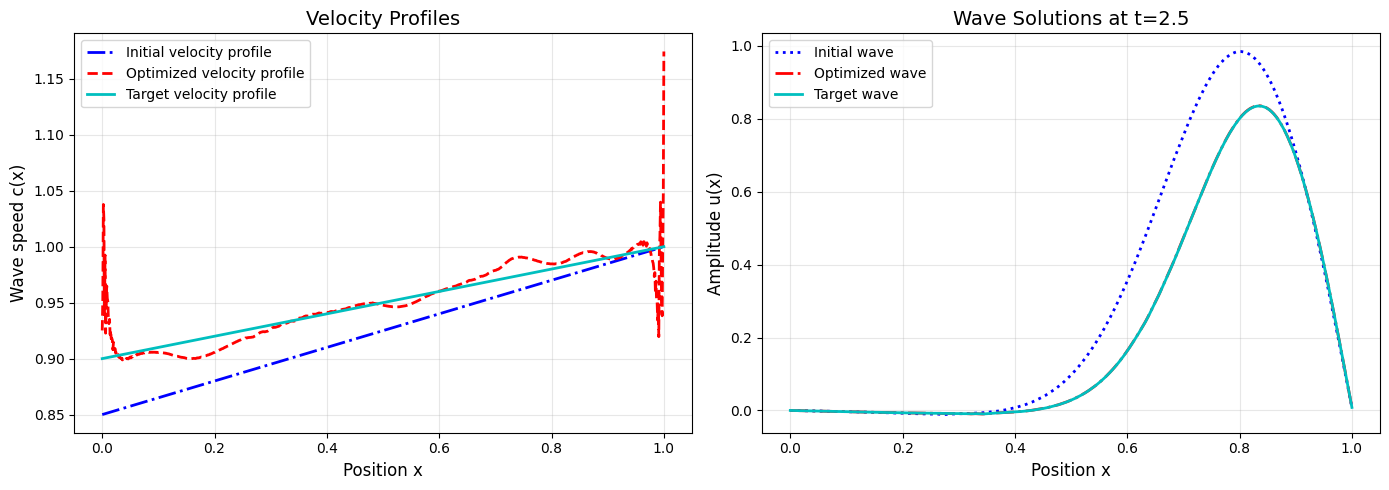
\includegraphics[width=\textwidth,height=0.46\textheight,keepaspectratio]{figs/fwi-linear-profile.png}
\end{center}
Adam takes 1000 steps with gradients from reverse mode, and the loss falls from 3.94 to 0.011.
The optimized wave lies on the target wave.
\medskip

Now look at the speed.
It follows the target along most of the column and oscillates near both ends.
Did the fit determine $c(x)$ everywhere?
\end{frame}

%------------------------------------------------
\section{From a Gradient to a Step}

%------------------------------------------------
\begin{frame}
\frametitle{A quadratic bowl}
So we have the gradient $\mathbf g_k=\nabla L(\mathbf x_k)$.
What step should we take?
Each optimizer replaces $L$ near $\mathbf x_k$ by a bowl in the step $\mathbf d$,
\[
q(\mathbf d)=\mathbf m^T\mathbf d+\tfrac12\,\mathbf d^TB\,\mathbf d,
\]
and moves to the bottom of the bowl, $\mathbf d=-B^{-1}\mathbf m$.
\begin{center}
\small
\begin{tabular}{llll}
\toprule
Optimizer & Slope $\mathbf m$ & Curvature $B$ & Step $\mathbf d$\\
\midrule
Gradient descent & $\mathbf g_k$ & $I/\eta$ & $-\eta\,\mathbf g_k$\\
Adam & $\hat{\mathbf m}_k$ & $\diag\big(\sqrt{\hat{\mathbf v}_k}+\epsilon\big)/\mathrm{lr}$ & $-\mathrm{lr}\,\hat{\mathbf m}_k/\big(\sqrt{\hat{\mathbf v}_k}+\epsilon\big)$\\
Newton & $\mathbf g_k$ & $\nabla^2L(\mathbf x_k)$ & $-[\nabla^2L(\mathbf x_k)]^{-1}\mathbf g_k$\\
L-BFGS & $\mathbf g_k$ & $H_k^{-1}$, from the last steps & $-t\,H_k\,\mathbf g_k$\\
\bottomrule
\end{tabular}
\end{center}
The optimizers differ in the slope and the curvature that they put into the bowl.
\end{frame}

%------------------------------------------------
\begin{frame}
\frametitle{The first step on a valley}
The loss is a narrow valley, $L=\tfrac12\,(x_1^2+64\,x_2^2)$, and every optimizer starts at $(-1.6,\,1.1)$.
\begin{center}
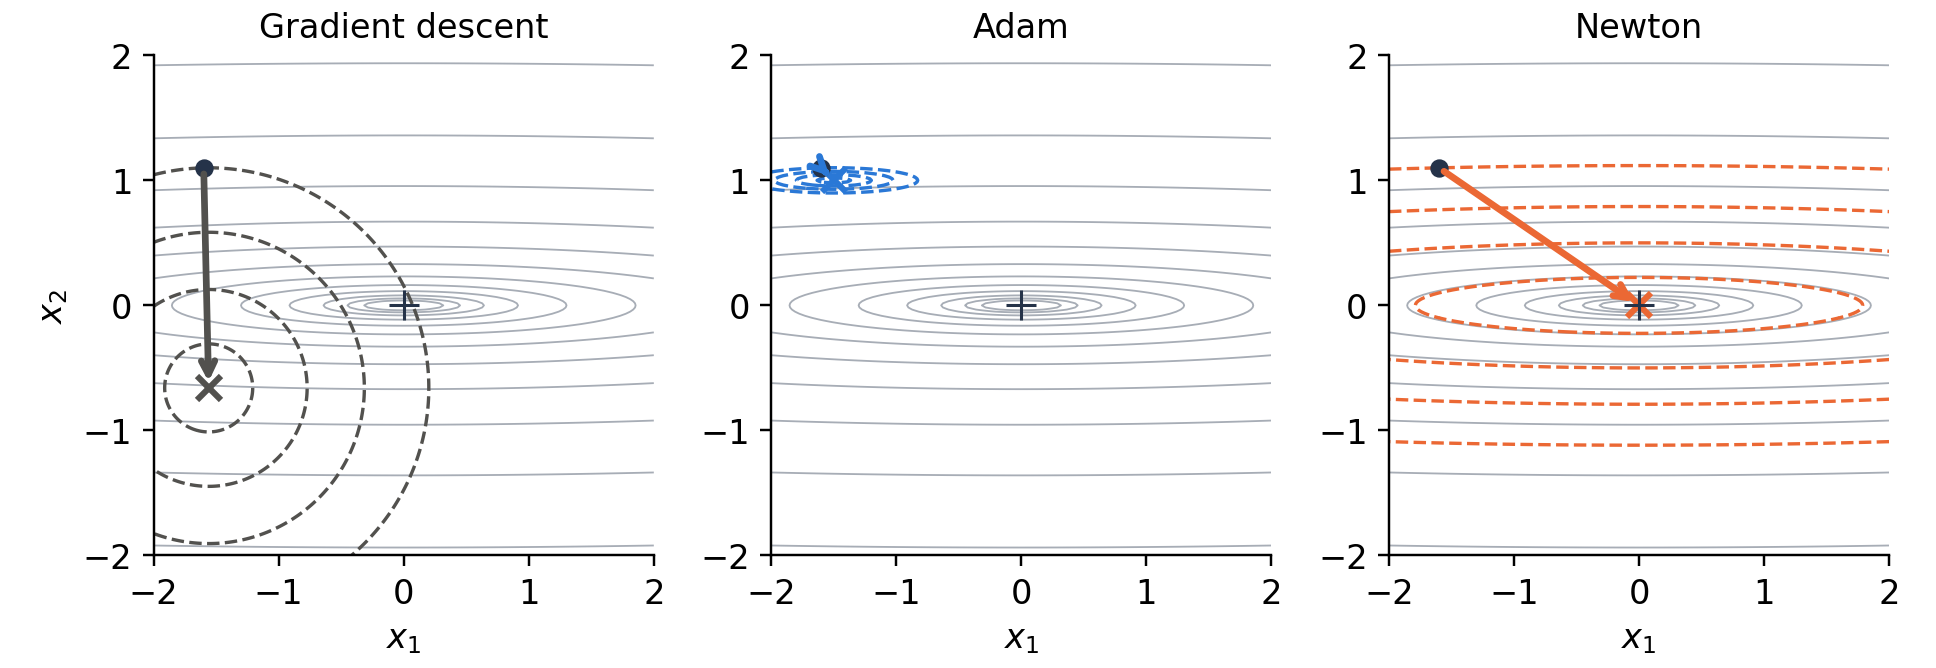
\includegraphics[width=\textwidth,height=0.4\textheight,keepaspectratio]{figs/three-bowls.png}
\end{center}
\small
The dashed curves are the bowl, the cross is its bottom, and the arrow is the step.
\smallskip

Gradient descent uses a round bowl, and its step $(0.04,\,-1.76)$ jumps across the valley floor.
Adam's bowl lines up with the axes, and its first step is $-\mathrm{lr}\,\sign(\mathbf g_1)=(0.1,\,-0.1)$.
Newton's bowl is the loss itself, so one step reaches the minimum.
\end{frame}

%------------------------------------------------
\begin{frame}
\frametitle{A narrow valley}
\begin{center}
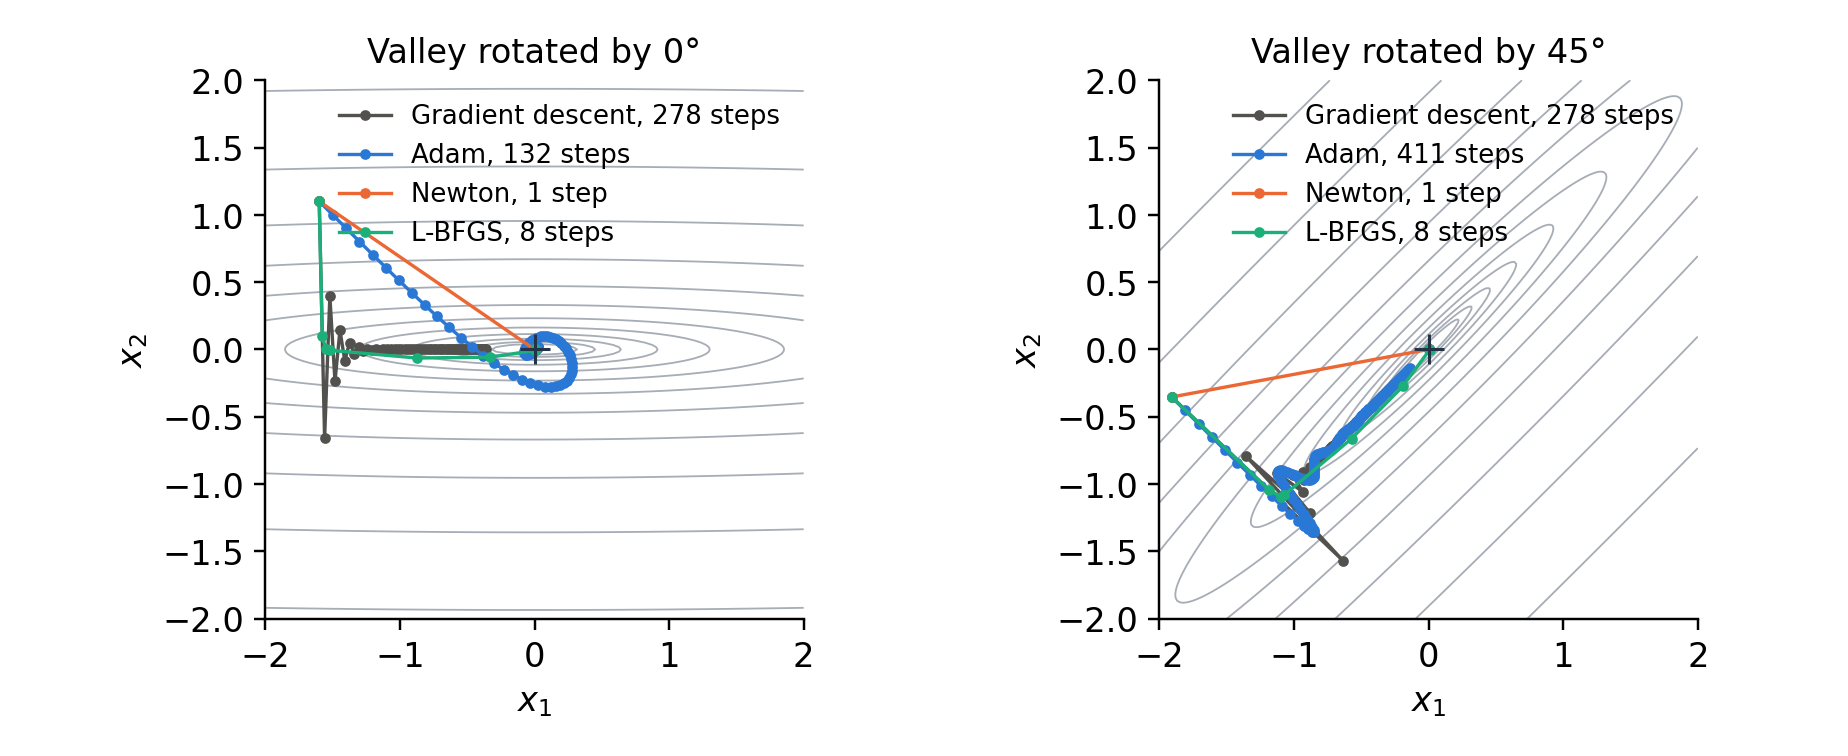
\includegraphics[width=\textwidth,height=0.47\textheight,keepaspectratio]{figs/valley-paths.png}
\end{center}
\small
The legends give the steps until $L<10^{-6}$, with $\eta=0.025$ and $\mathrm{lr}=0.1$.
\smallskip

Gradient descent is stable only for $\eta<2/64$, and with such an $\eta$ it creeps along the valley floor.
Adam rescales each coordinate and passes gradient descent, 132 steps against 278.
\smallskip

Now rotate the valley and the start by $45^\circ$.
Three paths repeat, rotated.
Adam's bowl stays lined up with the axes, and Adam needs 411 steps.
\end{frame}

%------------------------------------------------
\begin{frame}
\frametitle{Adam}
Adam averages the gradient and its square, coordinate by coordinate,
\[
\mathbf m_k=\beta_1\mathbf m_{k-1}+(1-\beta_1)\,\mathbf g_k,\qquad
\mathbf v_k=\beta_2\mathbf v_{k-1}+(1-\beta_2)\,\mathbf g_k^2 ,
\]
\[
\hat{\mathbf m}_k=\frac{\mathbf m_k}{1-\beta_1^k},\qquad
\hat{\mathbf v}_k=\frac{\mathbf v_k}{1-\beta_2^k},\qquad
\mathbf x_{k+1}=\mathbf x_k-\mathrm{lr}\,\frac{\hat{\mathbf m}_k}{\sqrt{\hat{\mathbf v}_k}+\epsilon}.
\]
The averages start at zero, and the division by $1-\beta^k$ removes that bias.
\bigskip

On the first step $\hat{\mathbf m}_1=\mathbf g_1$ and $\sqrt{\hat{\mathbf v}_1}=|\mathbf g_1|$, so every coordinate moves by $\mathrm{lr}$.
The size of the gradient and the units of the parameter cancel.
\bigskip

Adam divides each coordinate by its own scale.
It has no term that couples two coordinates, so a valley along a diagonal stays narrow.
\end{frame}

%------------------------------------------------
\begin{frame}
\frametitle{L-BFGS}
L-BFGS keeps the last $m$ steps $\mathbf s_i=\mathbf x_{i+1}-\mathbf x_i$ and gradient changes $\mathbf y_i=\mathbf g_{i+1}-\mathbf g_i$.
Each pair measures the curvature along one step, and $H_k$ satisfies $H_k\,\mathbf y_{k-1}=\mathbf s_{k-1}$.
\begin{center}
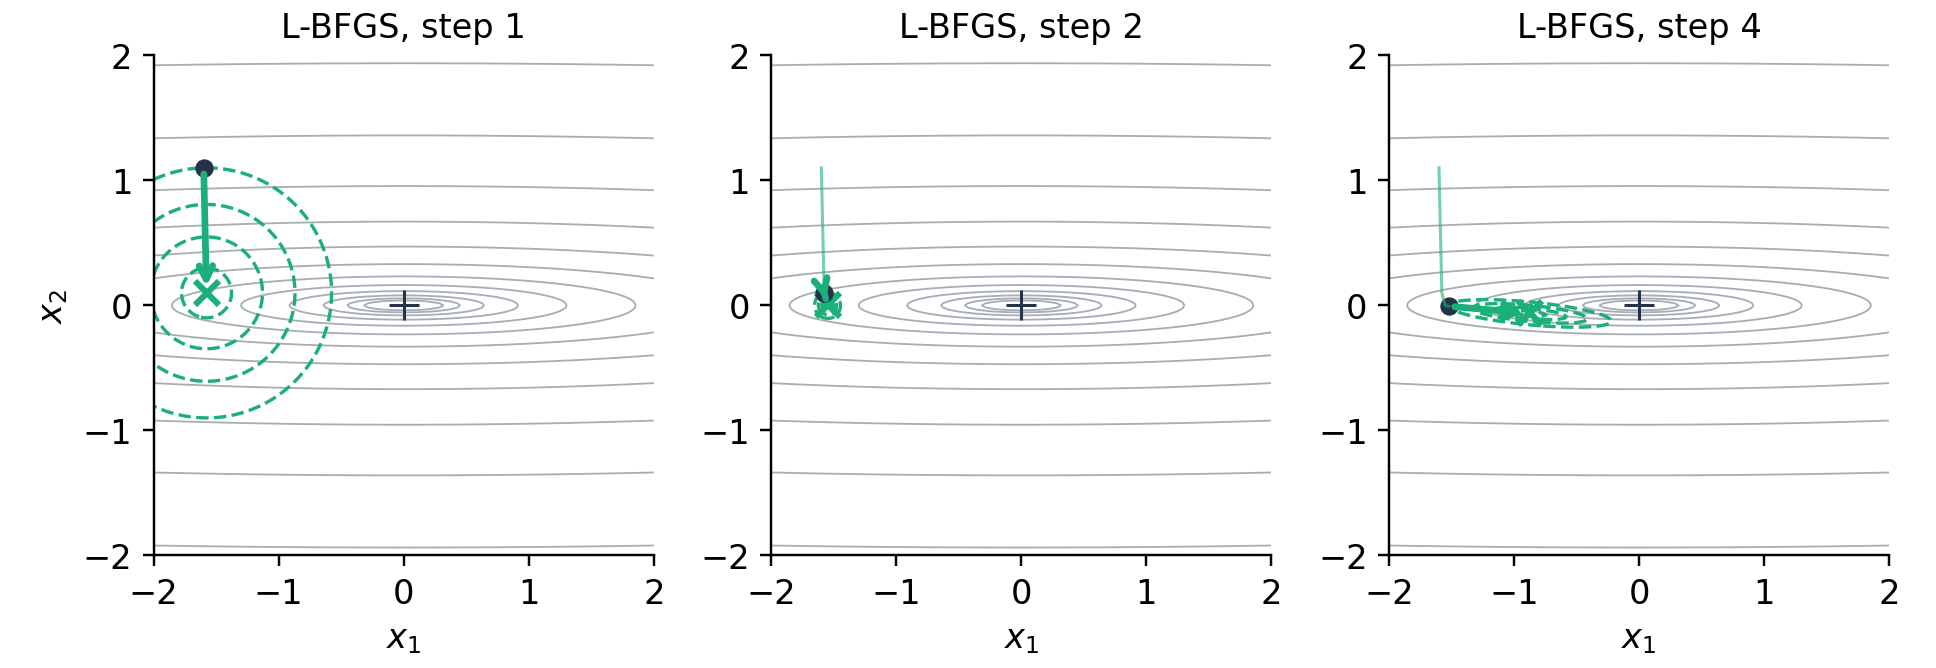
\includegraphics[width=\textwidth,height=0.38\textheight,keepaspectratio]{figs/lbfgs-bowls.png}
\end{center}
\small
The first bowl is round, with curvature 70 in every direction.
By step 4 the curvatures are 2.3 and 116, and the bowl lies along the valley, whose curvatures are 1 and 64.
\smallskip

The method stores $2mn$ numbers and never forms an $n\times n$ matrix.
A line search halves the step until the loss decreases enough.
\end{frame}

%------------------------------------------------
\begin{frame}
\frametitle{Rosenbrock and the double well}
\begin{center}
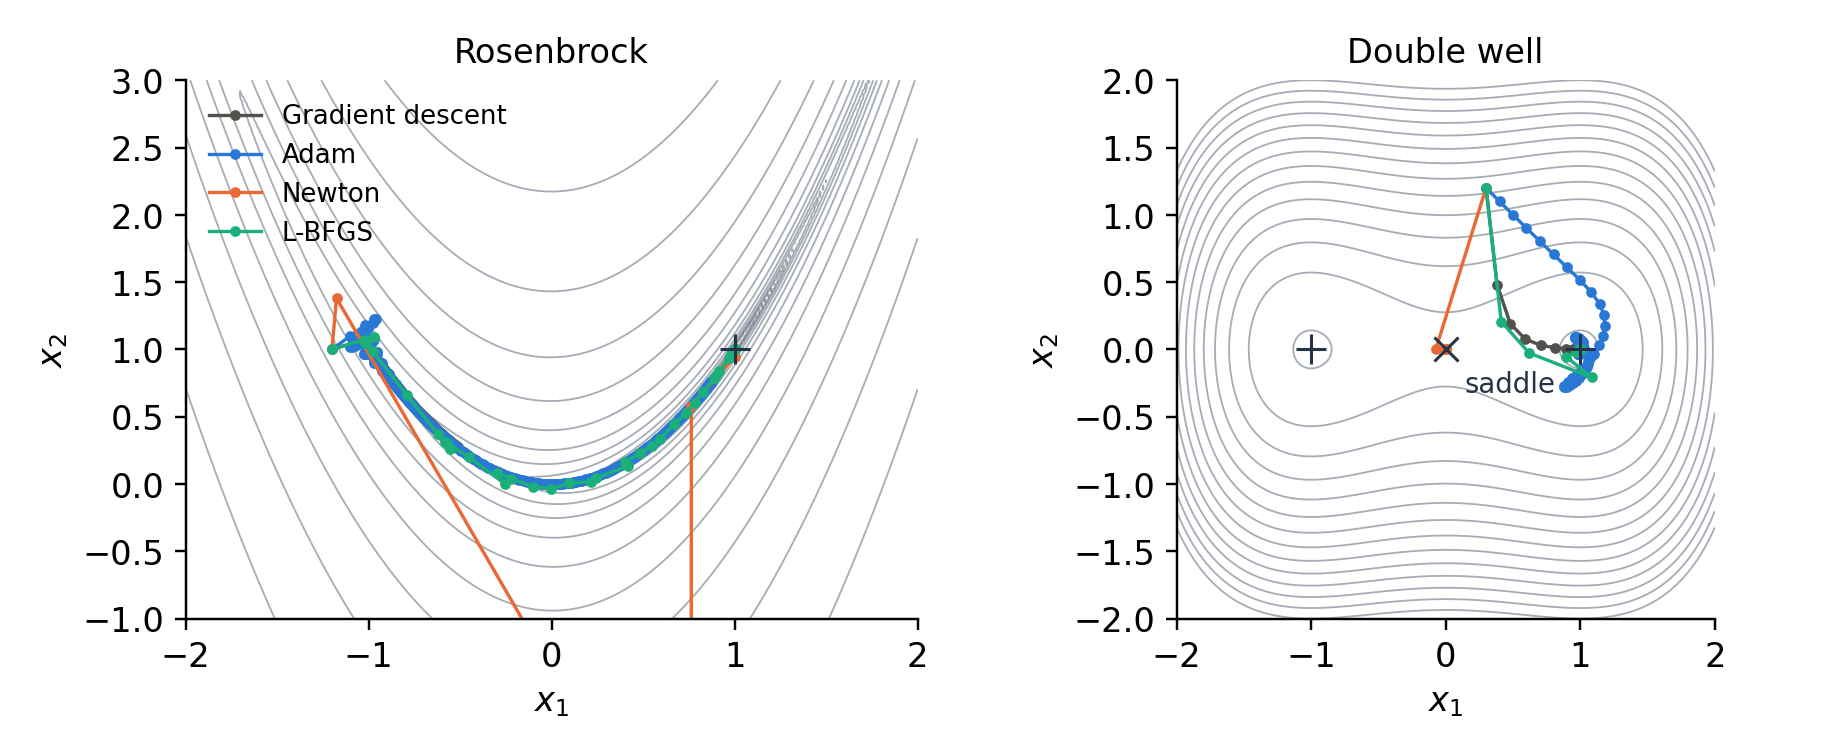
\includegraphics[width=\textwidth,height=0.48\textheight,keepaspectratio]{figs/rosenbrock-doublewell.png}
\end{center}
\small
On Rosenbrock, Newton reaches $(1,1)$ in 7 steps.
It has no line search, and its second step raises the loss from 4.7 to 1412.
L-BFGS arrives in 42 steps.
After 500 steps gradient descent is at $L=2.3$ and Adam at $L=0.016$.
\medskip

In the double well, the Hessian at the start has a negative eigenvalue, so Newton's bowl is a saddle.
Newton steps to the saddle point at the origin, where $L=0.25$, and stops.
The other three reach the minimum at $(1,0)$.
\end{frame}

%------------------------------------------------
\begin{frame}
\frametitle{Noisy gradients}
A minibatch gives a gradient with noise.
On the narrow valley, add Gaussian noise to every gradient, with a standard deviation of 5 percent of the size of the first gradient.
\begin{center}
\begin{tabular}{ll}
\toprule
Optimizer & 500 steps with noisy gradients\\
\midrule
Gradient descent & wanders about 0.42 from the minimum\\
Adam & wanders about 0.45 from the minimum\\
Newton & leaves the plot at step 22\\
L-BFGS & the line search fails at step 3\\
\bottomrule
\end{tabular}
\end{center}
The two distances are averages over the last 100 steps.
\medskip

Newton multiplies the noise by $[\nabla^2L]^{-1}$, which is 40 times the step size $\eta$ along the valley floor.
L-BFGS builds its curvature from differences of noisy gradients.
\medskip

Which of these methods can train a network on minibatches?
\note{Numbers from figs/src/page\_numbers.js, which runs the page's own code with its seeded noise (seed 7, sigma 0.05).}
\end{frame}

%------------------------------------------------
\begin{frame}
\frametitle{The optimizers compared}
\begin{center}
\small
\begin{tabular}{L{0.19\textwidth}L{0.25\textwidth}L{0.13\textwidth}L{0.28\textwidth}}
\toprule
Optimizer & Information per step & Extra memory & Slow or wrong when\\
\midrule
Gradient descent & one gradient & none & the curvature differs between directions\\
\addlinespace
Adam & one gradient and two running averages & $2n$ & the valley does not lie along the coordinate axes\\
\addlinespace
Newton & one gradient and one Hessian & $n^2$, and a linear solve & the Hessian is indefinite or singular, or $n$ is large\\
\addlinespace
L-BFGS & one gradient, loss values, and $m$ pairs & $2mn$ & the gradients are noisy\\
\bottomrule
\end{tabular}
\end{center}
\medskip
The memory is for $n$ parameters.
With a million parameters and minibatch gradients, which of these bowls can we still compute and store?
\end{frame}

%------------------------------------------------
\begin{frame}
\frametitle{A loss with a curve of minima}
\begin{columns}[T]
\begin{column}{0.5\textwidth}
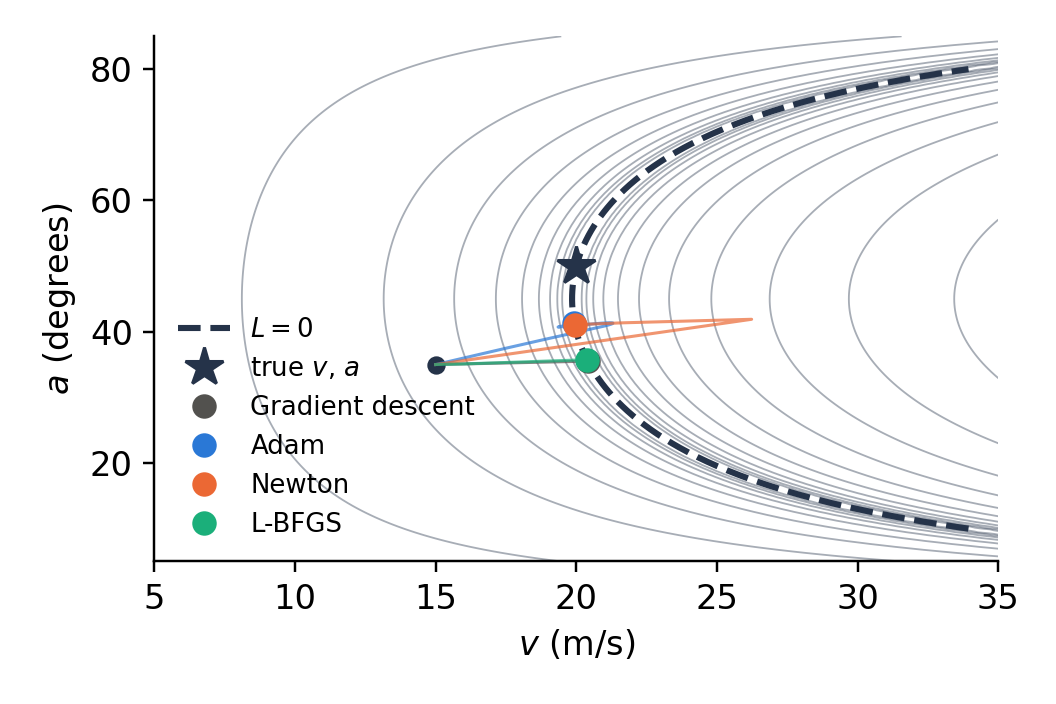
\includegraphics[width=\linewidth]{figs/landing-minima.png}
\end{column}
\begin{column}{0.48\textwidth}
\small
Now observe one number, the landing distance $R=v^2\sin 2a/g$.
\medskip

The loss is zero on the whole curve $v^2\sin 2a=g\,R^*$.
\medskip

\footnotesize
\begin{tabular}{@{}lcc@{}}
\toprule
Stops at & $v$ (m/s) & $a$\\
\midrule
Gradient descent & 20.41 & $35.5^\circ$\\
Adam & 19.93 & $41.3^\circ$\\
Newton & 19.94 & $41.1^\circ$\\
L-BFGS & 20.38 & $35.7^\circ$\\
\bottomrule
\end{tabular}
\medskip

\small
No optimizer returns the true $a=50^\circ$.
\end{column}
\end{columns}
\medskip
Every arc on the curve lands at the same distance.
A loss of zero leaves the parameters undetermined when the data cannot tell them apart.
\end{frame}

%------------------------------------------------
\section{Scale and Inverse Updates}

%------------------------------------------------
\begin{frame}
\frametitle{A simulator that scales one input}
Here is the simplest simulator that treats its inputs differently, $\mathbf y(\mathbf x)=(x_1,\ \alpha\,x_2)$, with the loss
\[
L=\lVert\mathbf y\rVert^2=x_1^2+\alpha^2x_2^2 .
\]
At $(1,1)$ with $\alpha=10$ the gradient is $(2,\,200)$, while the minimum lies along $-(1,1)$.
\begin{center}
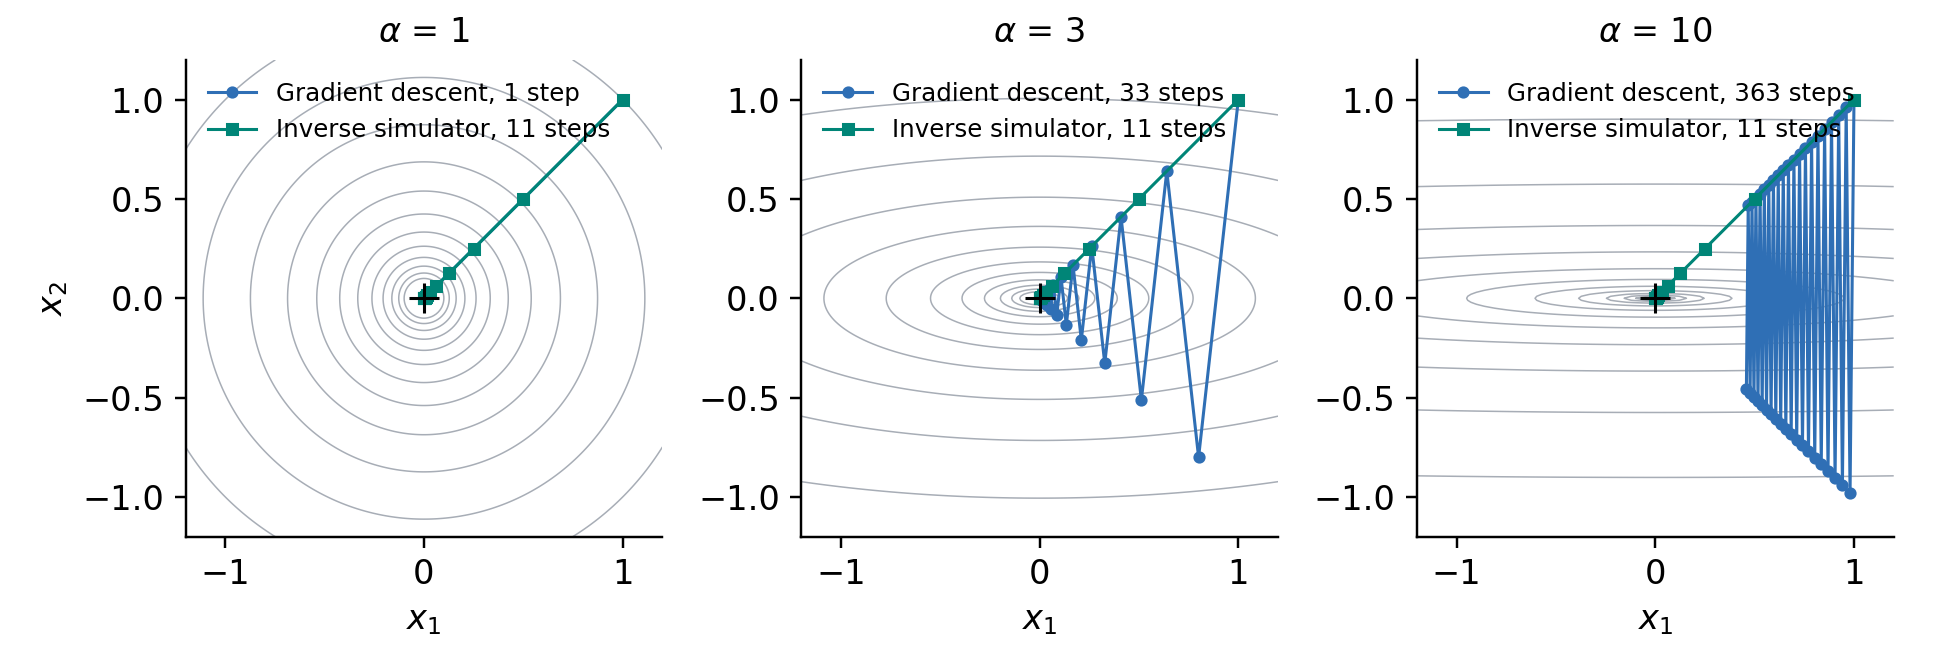
\includegraphics[width=\textwidth,height=0.33\textheight,keepaspectratio]{figs/scaled-simulator.png}
\end{center}
\small
Gradient descent with its best fixed step needs 1, 33, and 363 steps, and the count grows like $\alpha^2$.
Now invert the simulator.
Step toward the target in $\mathbf y$ and map the step back, $\mathbf x_{k+1}=\mathbf y^{-1}\big((1-\eta)\,\mathbf y(\mathbf x_k)\big)=(1-\eta)\,\mathbf x_k$.
The path is the same for every $\alpha$, so this update is \textbf{scale invariant}.
\end{frame}

%------------------------------------------------
\begin{frame}
\frametitle{A nonlinear simulator}
The example of Physics-based Deep Learning squares the second input,
\[
\mathbf y(\mathbf x)=\begin{bmatrix}x_1\\ x_2^2\end{bmatrix},\qquad L=\lVert\mathbf y\rVert^2,\qquad \mathbf x_0=(3,3).
\]
Reverse mode computes the gradient in two stages through $\mathbf y$.
It first finds $\partial L/\partial\mathbf y=2\mathbf y=(6,18)$, and then it multiplies by the transposed Jacobian $J=\diag(1,\,2x_2)$,
\[
\nabla_{\mathbf x}L=J^T\frac{\partial L}{\partial\mathbf y}
=\begin{bmatrix}1&0\\0&6\end{bmatrix}\begin{bmatrix}6\\18\end{bmatrix}
=\begin{bmatrix}6\\108\end{bmatrix}.
\]
The gradient points almost along $x_2$, although the minimum lies along the diagonal.
\bigskip

The loss grows like $x_2^4$.
It is steep in $x_2$ at the start and flat in $x_2$ near the minimum.
Which update copes with both?
\end{frame}

%------------------------------------------------
\begin{frame}
\frametitle{Gradient, Newton, and inverse updates}
Each update proposes a step $\Delta\mathbf x$.
The last two first choose a step in the output, $\Delta\mathbf y=-\eta\,\mathbf y$.
\begin{center}
\small
\begin{tabular}{llll}
\toprule
Update & Step $\Delta\mathbf x$ & Needs & New $x_2$\\
\midrule
Gradient descent & $-\eta\,\nabla_{\mathbf x}L$ & the gradient & $x_2-4\eta\,x_2^3$\\
Newton & $-\eta\,(\nabla^2_{\mathbf x}L)^{-1}\nabla_{\mathbf x}L$ & the Hessian in $\mathbf x$ & $(1-\eta/3)\,x_2$\\
Inverse gradient & $J^{-1}\Delta\mathbf y$ & $J$, inverted & $(1-\eta/2)\,x_2$\\
Inverse simulator & $\mathbf y^{-1}(\mathbf y+\Delta\mathbf y)-\mathbf x$ & a local inverse of $\mathbf y$ & $\sqrt{1-\eta}\;x_2$\\
\bottomrule
\end{tabular}
\end{center}
\medskip
The gradient step in $x_2$ is large far from the minimum and vanishes near it.
Newton divides the gradient entry $4x_2^3$ by the Hessian entry $12x_2^2$.
The inverse simulator shrinks $y_2$ by the factor $1-\eta$.
\medskip

The step sizes follow Physics-based Deep Learning, $\eta=0.01$ for gradient descent, $1/3$ for Newton, and $0.3$ for the two inverse updates.
\end{frame}

%------------------------------------------------
\begin{frame}
\frametitle{The paths of the updates}
\begin{center}
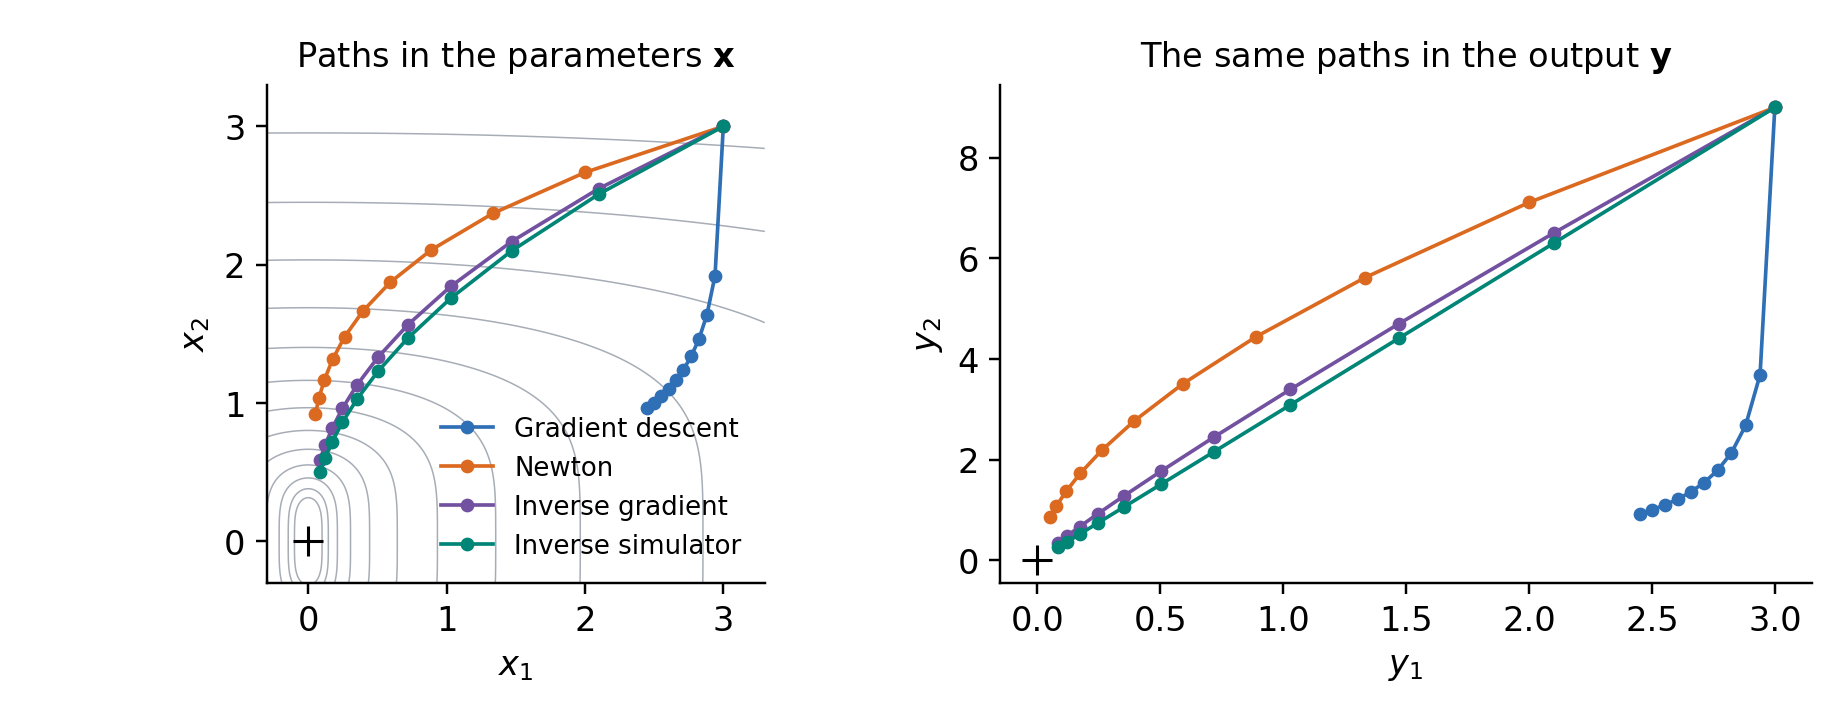
\includegraphics[width=\textwidth,height=0.45\textheight,keepaspectratio]{figs/four-updates.png}
\end{center}
\small
Distance to the minimum after 10 steps
\begin{center}
\begin{tabular}{cccc}
\toprule
Gradient descent & Newton & Inverse gradient & Inverse simulator\\
\midrule
2.633 & 0.925 & 0.597 & 0.511\\
\bottomrule
\end{tabular}
\end{center}
The first step of gradient descent is almost all in $x_2$, and then its steps in $x_2$ vanish like $x_2^3$.
Newton's $x_2$ shrinks by $8/9$ per step, because the Hessian entry also vanishes at the minimum.
The inverse simulator moves along a straight line in $\mathbf y$.
\end{frame}

%------------------------------------------------
\begin{frame}
\frametitle{The limits of inversion}
Inversion needs a square Jacobian that we can invert.
\bigskip

A network maps millions of weights to one loss.
Then $\partial L/\partial\bm\theta$ is a single row, and it has no inverse.
Physics-based Deep Learning keeps gradient descent for the weights and uses inverse steps for the physics.
\bigskip

An inverse can also exist and amplify noise.
Heat flow on a ring multiplies mode $k$ by $e^{-\nu k^2T}$, and its inverse multiplies mode $k$ by $e^{\nu k^2T}$.
With $\nu T=0.091$ the inverse factor at $k=12$ is $4.9\times10^5$.
A measurement error of $10^{-6}$ in that mode becomes an error of $0.5$ in the recovered initial temperature.
\bigskip

Where in a physics-based model can we use an inverse, and where must we fall back on the gradient?
\end{frame}

%------------------------------------------------
\section{Losses with Kinks}

%------------------------------------------------
\begin{frame}
\frametitle{Derivatives at a kink}
The function $|x|$ has slope $-1$ to the left of zero and $+1$ to the right, so it has no derivative at $x=0$.
The ReLU has a corner there too.
Ask PyTorch for the derivative at $x=0$.
\begin{center}
\begin{tabular}{lc}
\toprule
Function & Derivative returned at 0\\
\midrule
\texttt{torch.abs(x)} & 0\\
\texttt{torch.relu(x)} & 0\\
\texttt{torch.clamp(x, min=0)} & 1\\
\texttt{torch.maximum(x, 0)} & 0.5\\
\bottomrule
\end{tabular}
\end{center}
\medskip
The last three rows are the same function, written three ways.
Each library operation picks its own value at the corner.
\bigskip

Which of these values are correct?
\end{frame}

%------------------------------------------------
\begin{frame}
\frametitle{Subgradients}
\begin{center}
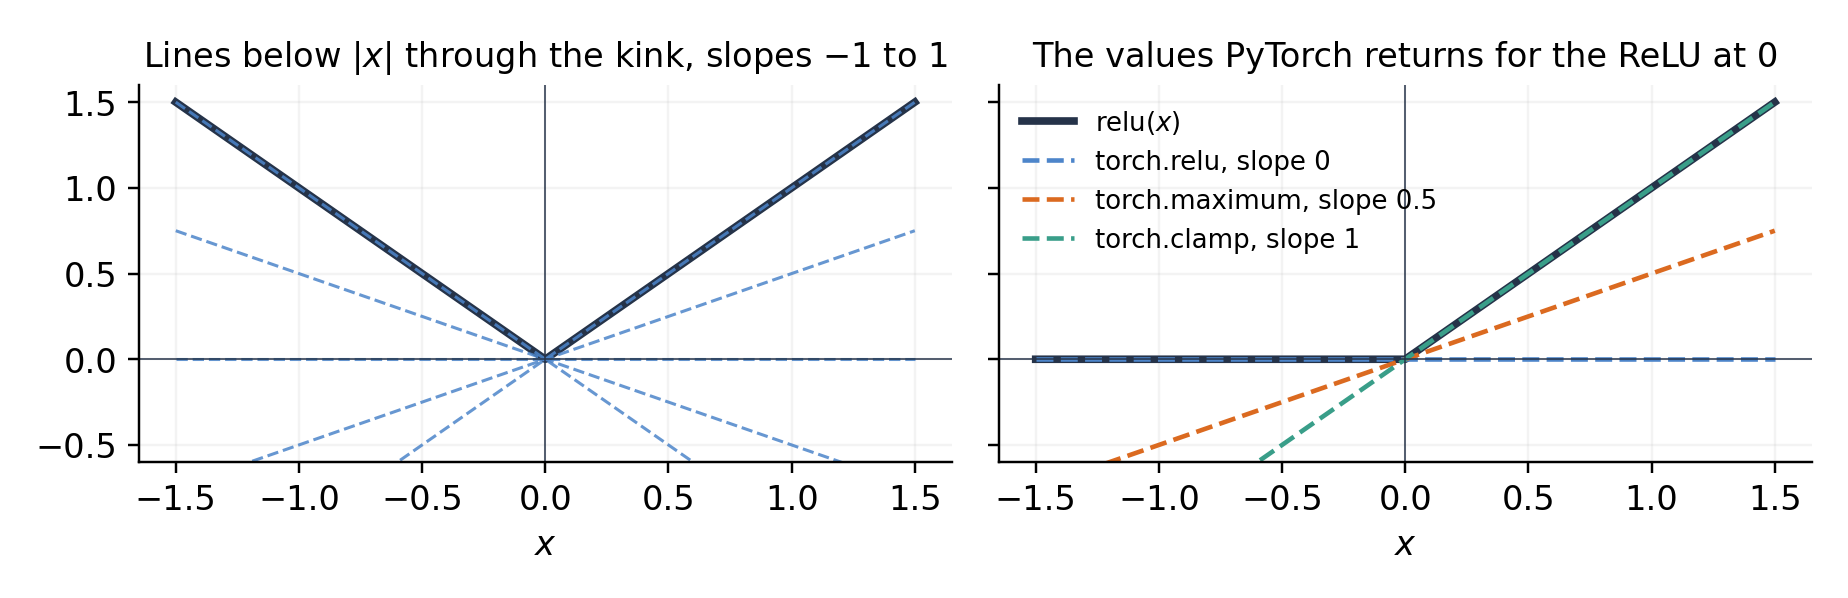
\includegraphics[width=\textwidth,height=0.42\textheight,keepaspectratio]{figs/subgradient-lines.png}
\end{center}
A number $g$ is a \textbf{subgradient} of a convex $f$ at $x$ when the line through $(x,f(x))$ with slope $g$ stays below the graph,
\[
f(z)\ge f(x)+g\,(z-x)\qquad\text{for every }z .
\]
The set of all subgradients is $\partial f(x)$.
At the kink, $\partial|x|=[-1,1]$ and $\partial\relu(x)=[0,1]$, so every value in the table is a subgradient.
\medskip

A point $x^\star$ minimizes a convex $f$ if and only if $0\in\partial f(x^\star)$.
\end{frame}

%------------------------------------------------
\begin{frame}
\frametitle{The subgradient method}
The obvious move copies gradient descent, $x_{k+1}=x_k-\eta_k\,g_k$ with $g_k\in\partial f(x_k)$.
Try it on $|x|$ from $x_0=1.05$.
\begin{center}
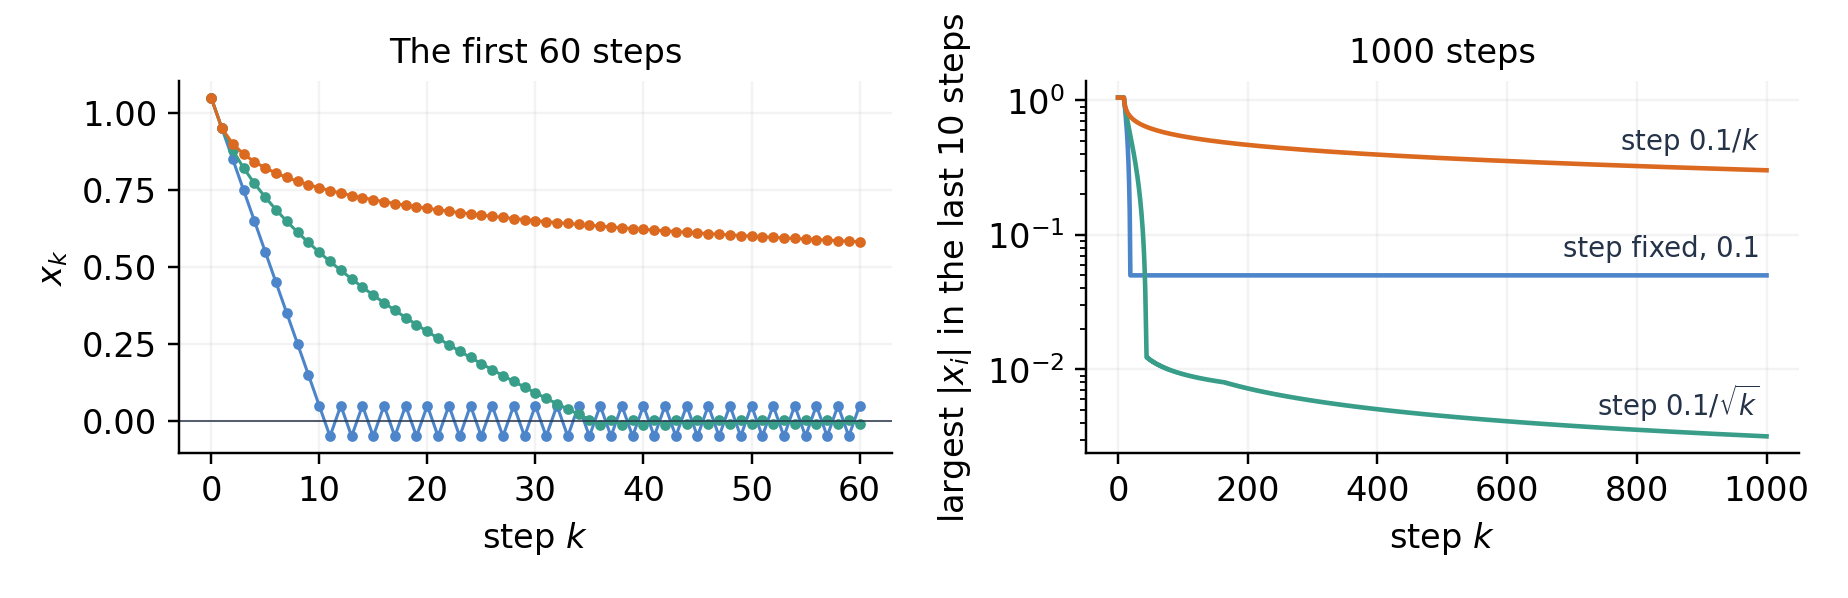
\includegraphics[width=\textwidth,height=0.36\textheight,keepaspectratio]{figs/subgradient-steps.png}
\end{center}
\small
The fixed step $0.1$ reaches $0.05$ in 10 steps and then jumps between $0.05$ and $-0.05$.
The subgradient has size 1 everywhere except at zero, so the step never shrinks.
\smallskip

With $\eta_k=0.1/\sqrt k$ the iterate lies within $0.0032$ of zero after 1000 steps.
With $\eta_k=0.1/k$ the steps add up to $0.75$, less than the starting distance, and the iterate stops at $0.30$.
The steps must shrink to zero, and their sum must still be infinite.
\end{frame}

%------------------------------------------------
\begin{frame}
\frametitle{The lasso}
The lasso fits a linear model with an $L^1$ penalty, $F(\mathbf w)=\frac{1}{2n}\lVert X\mathbf w-\mathbf y\rVert^2+\lambda\,\lVert\mathbf w\rVert_1$, here with 50 samples, 20 features, and $\lambda=0.1$.
\medskip

\small
The proximal gradient method takes a gradient step on the smooth part and then solves the kink in each coordinate, which gives the soft threshold $S_t(z)=\sign(z)\max(|z|-t,\,0)$.
\begin{center}
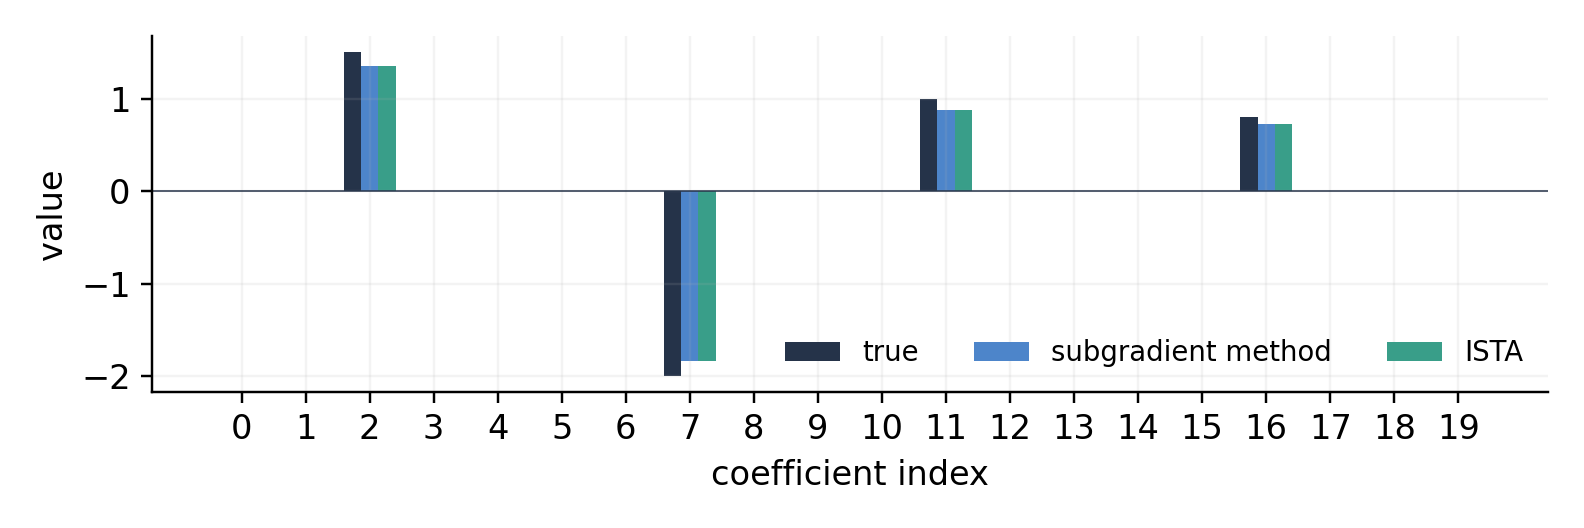
\includegraphics[width=0.95\textwidth,height=0.26\textheight,keepaspectratio]{figs/lasso-coefficients.png}
\end{center}
\begin{center}
\footnotesize
\renewcommand{\arraystretch}{0.9}
\begin{tabular}{lcc}
\toprule
Method & Objective $F$ & Coefficients equal to zero\\
\midrule
Subgradient method, 20000 steps & 0.50880 & 0\\
Proximal gradient, 5000 steps & 0.50876 & 15\\
scikit-learn \texttt{Lasso} & 0.50876 & 15\\
\bottomrule
\end{tabular}
\end{center}
\end{frame}

%------------------------------------------------
\begin{frame}
\frametitle{Kinks through the chain rule}
Automatic differentiation applies the chain rule with one chosen value at each kink.
For one kink that value is a subgradient.
A composition can break this.
\bigskip

\begin{center}
\begin{tabular}{lcc}
\toprule
Program & Subgradients at 0 & PyTorch returns\\
\midrule
$\relu(x)-\relu(-x)$, equal to $x$ & $\{1\}$ & 0\\
$\sqrt{x^2}$, equal to $|x|$ & $[-1,1]$ & \texttt{nan}\\
\bottomrule
\end{tabular}
\end{center}
\bigskip

In the first row the chain rule multiplies $\relu'(0)=0$ into both terms.
In the second row it evaluates $0/0$.
Away from the kink both programs get the correct derivative.
\bigskip

For programs built from the usual nonsmooth pieces, the output of AD differs from the derivative on a set of measure zero (Bolte and Pauwels, 2020).
\note{Kakade and Lee (2018) use a ReLU composition of this kind to show that AD libraries do not compute subgradients of compositions in general.}
\end{frame}

%------------------------------------------------
\begin{frame}
\frametitle{Further reading}
\begin{itemize}
\item Baydin, Pearlmutter, Radul, and Siskind (2018). Automatic differentiation in machine learning, a survey. \textit{Journal of Machine Learning Research} 18.
\item Griewank and Walther (2008). \textit{Evaluating Derivatives}, second edition. SIAM.
\item Nocedal and Wright (2006). \textit{Numerical Optimization}, second edition. Springer.
\item Kingma and Ba (2015). Adam, a method for stochastic optimization. ICLR.
\item Holl, Koltun, and Thuerey (2022). Scale-invariant learning by physics inversion. \href{https://arxiv.org/abs/2109.15048}{arXiv:2109.15048}, and \href{https://www.physicsbaseddeeplearning.org/physgrad.html}{Physics-based Deep Learning}.
\item Kakade and Lee (2018). Provably correct automatic subdifferentiation for qualified programs. \href{https://arxiv.org/abs/1809.08530}{arXiv:1809.08530}.
\item Bolte and Pauwels (2020). A mathematical model for automatic differentiation in machine learning. \href{https://arxiv.org/abs/2006.02080}{arXiv:2006.02080}.
\end{itemize}
\end{frame}

%------------------------------------------------
\begin{frame}
\frametitle{Questions?}
\centering
\Large
Thank you!
\vspace{1cm}

\normalsize
\textbf{Contact:} \\
Krishna Kumar \\
\textit{krishnak@utexas.edu} \\
University of Texas at Austin
\end{frame}

\end{document}
